% \addcontentsline{toc}{chapter}{Problem Implementation}
\chapter{Problem Implementation}
\oddsidemargin = -30pt

\section{Grammar}

\noindent For a better understanding, further is represented the grammar for this specific language according to a very simple and textual program. Through it, was shown in detail each feature of grammar.
The DSL design includes several stages. First of all, definition of the programming
language grammar  
G = (VN,VT, P, S ):

VN – is a finite set of non-terminal symbol;

VT - is a finite set of terminal symbols.

P – is a finite set of production of rules;

S - is the start symbol;\\

$VN = {<program>, <var>, <knot>, <ID>, <content>, <text>, <goto>, <print>,$
$<img>, <choice>, <var_op>, <expr>, <int>, <str>, <value>, <var_name>, $
$<knot_name>, <img_name>, <option_text>, <EQ>, <LPAREN>, <RPAREN>, <LCURLY>, $
$<RCURLY>, <GH>, <EXLAM>, <IMG_NAME>, <INT>, <ID>, <WS>, <EOF>} $

$VT = {'EOF', '(', ')', '*', '=', '<', '>', '[', ']', '{', '}', '!', '+', '-', '/', '(', ')(', ')', '<', '>', '=', '[', ']', '!', a'{', '}', ',', $
$'.png', '.jpg', ‘0’..’9’, ‘a..z’, ‘A’..’Z’}$

In Table \ref{tbl:meta}, meta-notations used for specifying the grammar are presented.

\begin{table}[h]
    \centering
    \begin{tabular}{|c|c|}
        \hline
        Notation (symbol) & Meaning\\
        \cline{1-2}
        $<foo>$ & means foo is a nonterminal\\
        \hline
        foo & foo in bold means foo is a terminal\\
        \hline
        x* & zero or more occurrences of x\\
        \hline
        $|$ & separates alternatives\\
        \hline
        $\rightarrow$ & derives\\
        \hline
        // & comment section\\
        \hline
    \end{tabular}
    \captionsetup{justification=centering} % Add this line after \begin{table}
    \caption{Meta Notation}
    \label{tbl:meta}
\end{table}


\begin{verbatim}
    
        grammar Expr;
        
        <program>: (<var>)* <knot>+ EOF;
        
        <knot> : <ID> '{' <content>* '}'; 
        <var>: <var_name> '=' <value>;
        <value>: <int>|<str>;
        <int>:<INT>;
        <str>:'"'(<ID>|<INT>)*'"';
        
        
        <content>: <text>
            | <goto>
            | <print>
            | <npc>
            | <choice>
            | <var_op>
            | <if>
            ;
        
        <var_op> : '[' <var_name> '=' <expr> ']';
        <if> : '(' '(' '?' <logic_expr> <goto> ')'')';
        
        <logic_expr>: <logic_expr> ('&''&'|'|''|') <logic_expr>
                   | '(' <logic_expr> ')'
                   | <bool_expr>
                    ;
        <bool_expr>: <bool_expr> ('>'|'<'|'!''='|'=''='|'>''='|'<''=') <bool_expr>
                   | <expr>
                   ;
        
        <expr>:   <expr> ('*'|'/') <expr>
            |   <expr> ('+'|'-') <expr>
            |   <int>
            |   '(' <expr> ')'
            |   <str>
            | <var_name>
            ;
        
        <goto> : '(' <knot_name> ')' ;
        <print> : '(''(' <var_name> ')'')';
        <npc>: '(''!' (<text>)+ ')';
        <choice>: '(' '(' <pair*>  ')'')';
        <pair>:'!'(<text>)+ <goto>;
        <knot_name>: <ID>;
        <var_name>:<ID>|<INT>;
        <text>: <ID>|<INT>;
        
        <EQ> : '=' ;
        <LPAREN> : '('; 
        <RPAREN> : ')' ;
        <LCURLY> : '{' ;
        <RCURLY> : '}' ;
        <GH>:'"';
        <EXLAM>: '!';
        <L>: '[';
        <R>: ']';
        <MULT>: '*';
        <DIVIDE>: '/';
        <SUB>: '-';
        <ADD>: '+';
        
        INT : [0-9]+ ;
        ID: [a-zA-Z_0-9?.\\,;%<>!]+; 
        WS: [ \t\n\r\f]+ -> skip ;
\end{verbatim}


\section{Semantic and lexicon}
\noindent The grammar provided is a context-free grammar (CFG) that defines the syntax rules for an interactive story telling program. Here are the descriptions of the semantic and lexicon of the grammar:\\
Semantic:
\begin{itemize}
        \item $<program>$ is the starting point of the program, which consists of a series of $<var>$ declarations followed by one or more $<knot>$ definitions.
        \item $<knot>$ defines a scene or a chapter in the story, identified by an $<ID>$ (identifier) followed by a block of $<content>$ that can be a sequence of text, choices, images, variables, and go-to statements.
        \item $<var>$ declares a variable with a $<var_name>$ identifier and assigns a $<value>$ to it, where a value can be either an integer or a string.
        \item $<var_op>$ is an expression that can update the value of a variable by performing basic arithmetic operations on it.
        \item $<expr>$ is an arithmetic expression that can include integers, strings, and variables. \\
\end{itemize}
Lexicon:
\begin{itemize}
        \item $<INT>$ is a regular expression that represents any positive integer number.
        \item $<ID>$ is a regular expression that represents an identifier or a name, starting with an alphabetical character or an underscore and followed by alphanumeric characters or underscores.
        \item $<IMG_NAME>$ is a regular expression that represents the name of an image file in the PNG or JPG format.
        \item $<WS>$ is a regular expression that matches any whitespace character and is ignored by the parser.
        \item $<EQ>, <LPAREN>, <RPAREN>, <LCURLY>, <RCURLY>, <GH>, and <EXLAM>$ are tokens that represent the symbols "=","(",")","{","}","""","!" respectively, used to separate and define the syntax rules of the grammar.
\end{itemize}

\section{Syntax Analysis}
Writing syntax analysis for an interactive storytelling language involves creating a grammar that defines the language's syntax and using it to parse input text to ensure it conforms to the grammar rules. We started by defining the language’s grammar, then we generated the parser, using ANTLR, that was able to read and interpret the input text according to the grammar rules. Afterwards the parser has successfully recognized a valid input, it needs to perform semantic actions based on the syntax to actually execute the code. This involves interpreting the input and manipulating variables, objects, or other data structures as necessary. For our interactive storytelling language, these semantic actions were changing the storyline based on user choices or triggering events based on certain input. Therefore, we had only to handle the errors, test and refine the grammar and parser as needed to improve accuracy of performance.

Creating syntax analysis for our interactive storytelling language was like putting together a detailed puzzle. It started with us drafting a grammar that laid out the rules for the language's syntax. Think of it as the blueprint for how the language should work. Once we had our blueprint in place, we used it to parse input text, kind of like a filter, to make sure it followed our rules.

Then came ANTLR, a super handy tool that we used to generate our parser. The parser's job was to read and interpret the input text, like a guide navigating a map, using the grammar rules we set up. It was like having a translator who could decode our language into something the computer could understand and work with.But recognizing valid input wasn't the end game. After that, the parser needed to do something with the input - this is where semantic actions came in. In our case, these actions involved altering the storyline based on user choices or setting off certain events based on the input. So, if a user made a choice in our interactive story, the parser would kick into action and change the story's direction accordingly.

The last part of our journey involved a lot of testing, refining, and error handling. We had to make sure our grammar and parser were as accurate as possible, and that meant going back to the drawing board several times. Like any good piece of work, it was all about trial and error, and constant refining to ensure the best performance.

\section{Code Explanation}
Lexer and parser classes are automatically generated using the ANTLR4 tool, based on a grammar file provided. These classes are then imported into the main file.
\\In the main function, the source code is first passed to the lexer, which tokenizes the input. The tokenized output is then passed to the parser, which generates a parse tree based on the grammar rules defined in the grammar file.
\begin{verbatim}
        def main(argv):
        input_stream = InputStream(format_code(argv[1]))
    
        lexer = ExprLexer(input_stream)
        lexer.removeErrorListeners()
        lexer.addErrorListener(MyErrorLexerListener())
    
        stream = CommonTokenStream(lexer)
        parser = ExprParser(stream)
        parser.removeErrorListeners()
        parser.addErrorListener(MyErrorParserListener())
        tree = parser.program()
        
\end{verbatim}


\noindent Once the parse tree is generated, it is passed to the Interpreter class, which is manually implemented and not generated automatically like the lexer and parser. The Interpreter class performs further processing on the parse tree.
\begin{verbatim}
            tj = Interpreter(tree)
        
            tj.execute()
            
\end{verbatim}


\noindent The execute function within the Interpreter class follows a specific sequence of steps. First, it examines all declared variables at the top of the program and stores them in a dictionary for reference.
\\In the second step, the execute function selects the first knot declared in the code as the starting point:
\begin{verbatim}
            def execute(self):
            self.getVars()
            # starting knot is considered knot number 0
            start_knot = self.getKnotByIndex(0)
    
            self.checkKnot(start_knot)
            
\end{verbatim}

\noindent The checkKnot function within the execute function iterates over the content of each knot in a while loop. If it encounters a "go to" knot, it prints the text before that knot and proceeds to check the next knot in a similar manner.The checkKnot function within the execute function iterates over the content of each knot in a while loop. If it encounters a "go to" knot, it prints the text before that knot and proceeds to check the next knot in a similar manner.
\\These steps provide a formal outline of the process followed by the interpreter in executing the program.
\section{Parse Tree}
        A parsing tree or concrete syntax tree is an ordered, rooted tree that describes the syntactic structure of a string according to a context-free grammar. Computational linguistics is the main field in which the term "parse tree" is used. 
        The phrase "syntax tree" is more prevalent in theoretical syntax. The matching parse tree for the following sample of code was created (Fig. 1):
        
        \begin{verbatim}
                myvar="hello world"
                second=12
                f {
                        ce faci132
                        (y2)
                        ((j))
                        (!car.jpg)
                        ((!what are you doing (y2)
                        !here (y4)))
                    
                }
                
                y{
                hi io hi
                }     
        \end{verbatim}
        
        % { \centering 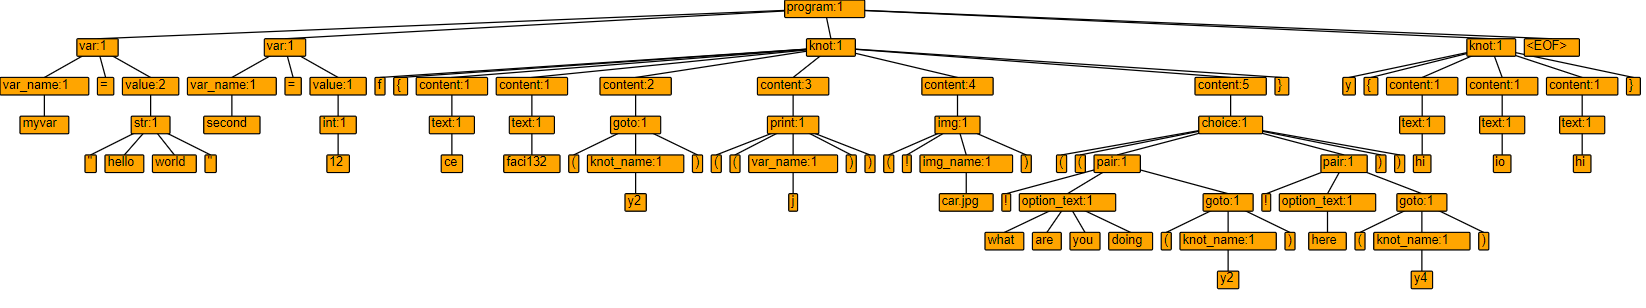
\includegraphics[width=\textwidth]{images/parsetree.png} }

\begin{figure}[h]
    \centering
    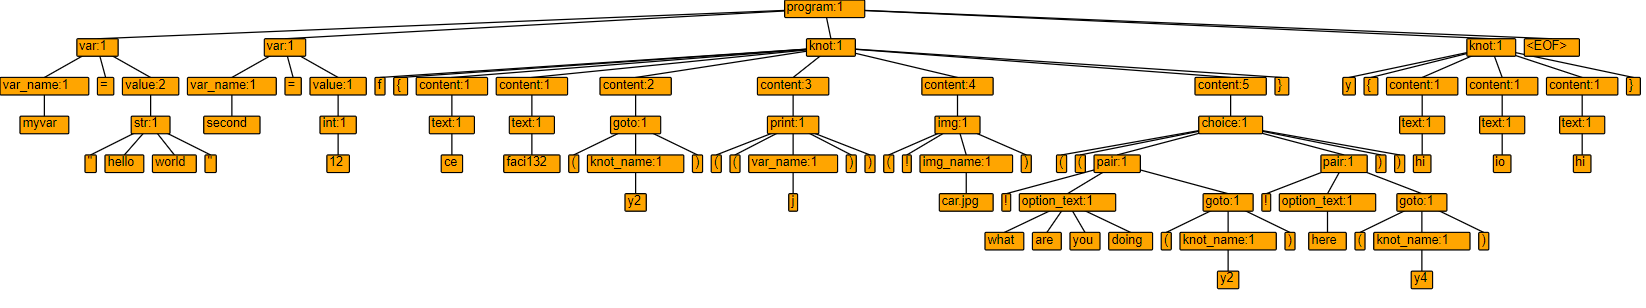
\includegraphics[width=\textwidth]{images/parsetree.png}
    \caption{Parse tree}
    \label{fig:parsetree}
\end{figure}

\section{Error handling}

In a DSL for interactive storytelling, there are several ways that programs might go wrong. Here are some examples:
\begin{itemize}
                \item \textbf{Data errors:} when the program manipulates data in unexpected ways, such as by accessing data that has not been initialized or by trying to perform an operation on incompatible data types.
                \item \textbf{Logic errors:} Logic errors occur when the program's code does not correctly reflect the intended logic of the story. For example, a branching structure might not accurately evaluate the reader's choices or a loop might not correctly repeat the desired actions.
                \item \textbf{Error messages:} The program might display an error message to the user, explaining what went wrong and how to fix it. This could include specific details about the error, such as which line of code caused the error or which input was invalid.
                \item \textbf{Debugging tools:} The DSL might provide debugging tools to help the user identify and fix errors. This could include features like step-through debugging, where the user can step through the code line-by-line and inspect the values of variables and data structures.
                \item \textbf{Tokenizer Errors:} An example of an error that can occur during tokenization is when an unrecognized character or symbol is encountered. If the input contains an invalid token that is not defined in the grammar, the lexer will raise an error. Here's a formal example:
                \\Input: "var1 = 10 \$ var2 = 20" Exception: TokenizationError: When tokenizing line 1, column 10: Token recognition error at: `\$`.
                \\In this example, the dollar sign ('\$') is not a valid character according to the defined grammar rules. The TokenizationError indicates the presence of an unrecognized character and provides the line number and column where the error occurred.
                \item \textbf{Parsing Errors:} A parsing error occurs when the input does not adhere to the grammar rules specified in the parser. Here's a formal example:
                \\Input: "var1=20 var2 10" Exception: ParsingError: When parsing line 1, column 13: No viable alternative at input 'var210'
                \\In this example, the second statement "var2 10" does not include the '=' sign, violating the grammar rules. The ParsingError indicates that the parser encountered a mismatched input error, expecting a semicolon (';') after the 'var2' identifier.
                \item \textbf{Variable Not Declared Error:} If you attempt to use a variable that has not been declared, you will encounter an error during runtime. Here's a formal example:
                \\Input: o=8 start { ((j)) } 
                \\Error: NotDeclaredVariable: Variable 'j' has not been declared, at line 5, column 6
                \\In this case, the variable 'j' has not been declared, resulting in a NotDeclaredVariable error when trying to print it.
                \item \textbf{Cannot Perform Mixed Operations Error:} Cannot Perform Mixed Operations Error: 
                \\Input: a="00" b=100 start { [b=a+100] } Error: CannotPerformMixedOperations: Cannot perform mixed operations, at line 4, column 7
                \\In this example, attempting to add a string ('a') with an integer ('100') leads to a CannotPerformMixedOperations error.
                \item \textbf{Not Valid Operation on String Error:} Performing arithmetic operations such as '*', '/', or '-' on strings is not valid and will produce an error. Here's a formal example:
                \\Input: a="00" start { [a=a-"0"] } Error: NotValidOperationOnString: Cannot perform '-' on strings, at line 3, column 7
                \\In this case, the operation of subtracting ("0") from a string ('a') is not valid and results in a NotValidOperationOnString error.
 \end{itemize}
 
\noindent These examples demonstrate various error scenarios, including tokenizer errors, parsing errors, variable not declared errors, mixed operations errors, and invalid string operations errors.
 \section{User Guide}

 \noindent For an easier way to use the presented domain specific language, all the functions will be broken down into pieces and explained alongside examples of code. 

 \noindent \textbf{Step 1: Variable Declaration}
 \begin{itemize}
                \item 	Variables are declared at the top of the knots.
                \item Each variable declaration consists of the variable name on the left-hand side, followed by an equal sign, and the value on the right-hand side.
                \item Each variable declaration consists of the variable name on the left-hand side, followed by an equal sign, and the value on the right-hand side.
                \item Example 
                        \begin{verbatim}
                        a = 4
                        b = 52
                        c = "Hello World"
                        start{
                        }

                        \end{verbatim}
                
 \end{itemize}

\noindent The declaration of variables is done in an intuitive way, as it can be seen in the example. Different values can be assigned to variables to store data. Variables are declared at the top of the knots. Each variable declaration consists of the variable name on the left-hand side, followed by an equal sign, and the value on the right-hand side. Strings are sequences of characters enclosed within quotation marks, so in this case c is assigned the string value of “Hello World”. 

  \noindent \textbf{Step 2: Knot declaration}
 \begin{itemize}
                \item Each knot is declared with a knot name followed by the content within curly brackets.
                \item Example: \begin{verbatim}
                        name_of_the_knot {
                        }
                        start{
                        }
                        Next_knot{
                        }
                        Ending{
                        }
                
                      \end{verbatim}
 \end{itemize}

\noindent Pieces of content are called knots. In order to allow the game to branch we need to markup sections of content with names. Each knot has to have a unique name and within each knot, it would be written the actual code or instructions that should be executed at that particular point in the program. Each knot is declared with a knot name followed by the content within curly brackets.

  \noindent \textbf{Step 3: Printing Variables}
 \begin{itemize}
                \item To print a variable, enclose the variable name within double open and close brackets.
                \item Example: \begin{verbatim}
                    	((var_name))
                      \end{verbatim}
 \end{itemize}


  \noindent \textbf{Step 4: Variable Declaration}
 \begin{itemize}
                \item The text in the knot doesn't need to be enclosed in any brackets; it can be plain text.

 \end{itemize}

   \noindent \textbf{Step 5: Dynamic Text}
 \begin{itemize}
                \item To include text that changes each time the program runs, enclose the text within open and closed brackets with an exclamation mark at the beginning.
                \item Example: \begin{verbatim}
                        (! This text is gonna change wow)
                      \end{verbatim}
 \end{itemize}


   \noindent \textbf{Step 6: Operations with Variables}
 \begin{itemize}
                \item Perform operations with variables using square brackets.
                \item On the left-hand side of the square brackets, specify the variable where the result will be stored.
                \item On the right-hand side, provide the expression to be calculated.
                \item Example: \begin{verbatim}
                        [b = 100 + 10 * (o / 4)]
                      \end{verbatim}
 \end{itemize}


   \noindent \textbf{Step 7: Transition to Other Knots}
 \begin{itemize}
                \item To move to another knot, enclose the name of the knot within a single open and closed bracket.
                \item The example shows the effortless way of including one knot inside another one, by simply adding its name inside the parenthesis: \begin{verbatim}
                        name_of_the_knot {
                    ( another_knot )
                    }
                    another_knot{
                    …
                    }                 









                    
                      \end{verbatim}
                   
 \end{itemize}
 
   \noindent \textbf{Step 8:  Choices}
 \begin{itemize}
                \item Choices are enclosed within double open and closed brackets.
                \itemEach choice starts with an exclamation mark, followed by the choice text, and then the "go to" knot.
                \item Example: \begin{verbatim}
                        start{
                        ((!save Joe (saveJoe)
                        !kill Joe (killJoe) ))
                        }
                        saveJoe{
                        }
                        killJoe{
                        }
                      \end{verbatim}
 \end{itemize}

 \noindent Input is offered to the player via text choices. A text choice is indicated by an ‘!’ character. If no other flow instructions are given, once made, the choice will flow into the next line of text. As for the above example the code snippet outlines a basic program structure where Joe can be saved or killed based on certain choices made.

    \noindent \textbf{Step 9: IF - conditional statement}
 \begin{itemize}
                \item This is the condition whose truth should be checked ‘((1=1 and 2+a>=4) or 1!=1?)’ and the ‘(end)’ block of code will be performed. Therefore, the if-else statement will execute the code within the end block, which is the phrase "I am smart” (assuming a is 2 or greater).
                \item Example: \begin{verbatim}
                        start{
                        ((1=1 and 2+a>=4) or 1!=1?(end))
                        }
                        end{
                        I am smart
                        }
                        
                      \end{verbatim}
 \end{itemize}